\documentclass{article}
\usepackage{amsmath} 
\usepackage{amsfonts} 
\usepackage{amssymb} 
\usepackage{graphicx}


\title{Integral Calculus}
\author{Kensukeken}
\date{July 29th, 2024}

\begin{document}

\maketitle
\tableofcontents
\newpage 

\section{Chapter 1}
\subsection*{Integrations}
Calculus is built on two operations — differentiation and integration. 
\begin{itemize}
  \item Differentiation — as we saw last term, differentiation allows us to compute and study the instantaneous rate of change of quantities. At its most basic it allows us to compute tangent lines and velocities, but it also led us to quite sophisticated applications including approximation of functions through Taylor polynomials and optimisation of quantities by studying critical and singular points. 
  \item Integration — at its most basic, allows us to analyse the area under a curve. Of course, its application and importance extend far beyond areas and it plays a central role in solving differential equations.
\end{itemize}
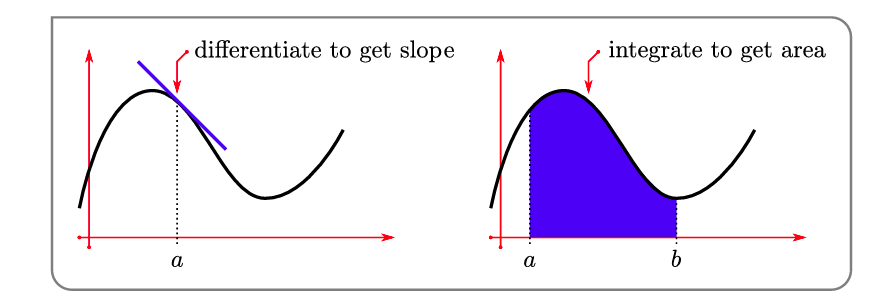
\includegraphics{./imgs/integral.png}

It is not immediately obvious that these two topics are related to each other. However, as weshall see, they are indeed intimately linked.



\section{Definite Integrals}

A definite integral is an integral with specified upper and lower limits. It is denoted as:
\[
\int_{a}^{b} f(x) \, dx
\]
where \(a\) and \(b\) are the limits of integration, and \(f(x)\) is the integrand.

\subsection{Fundamental Theorem of Calculus}

The Fundamental Theorem of Calculus connects differentiation and integration. It has two main parts:
\begin{itemize}
    \item \textbf{First Part:} If \(F\) is an antiderivative of \(f\) on \([a, b]\), then:
    \[
    \int_{a}^{b} f(x) \, dx = F(b) - F(a)
    \]
    \item \textbf{Second Part:} If \(f\) is continuous on \([a, b]\), then the function \(F\) defined by:
    \[
    F(x) = \int_{a}^{x} f(t) \, dt
    \]
    is continuous on \([a, b]\) and differentiable on \((a, b)\), and:
    \[
    F'(x) = f(x)
    \]
\end{itemize}

\section{Indefinite Integrals}

An indefinite integral represents a family of functions and is denoted as:
\[
\int f(x) \, dx
\]
It is also known as the antiderivative of \(f(x)\). The result includes an arbitrary constant \(C\):
\[
\int f(x) \, dx = F(x) + C
\]

\subsection{Basic Integration Rules}

\begin{itemize}
    \item \textbf{Power Rule:} For \(n \neq -1\):
    \[
    \int x^n \, dx = \frac{x^{n+1}}{n+1} + C
    \]
    \item \textbf{Constant Multiple Rule:} For a constant \(k\):
    \[
    \int k f(x) \, dx = k \int f(x) \, dx
    \]
    \item \textbf{Sum Rule:} For functions \(f(x)\) and \(g(x)\):
    \[
    \int [f(x) + g(x)] \, dx = \int f(x) \, dx + \int g(x) \, dx
    \]
\end{itemize}

\section{Applications}

Integral calculus is used to calculate areas under curves, volumes of solids of revolution, and other quantities. For example, to find the area under a curve \(y = f(x)\) from \(x = a\) to \(x = b\), we use the definite integral:
\[
\text{Area} = \int_{a}^{b} f(x) \, dx
\]

\end{document}
